\documentclass[a4paper]{article}
<<<<<<< HEAD

\begin{document}

\title{\Huge{Software Requirement Specification}}
\author{Group 8}
\maketitle

\section{Introduction}

The purpose of this document is to present a detailed description for the mark record and tracking solution. It will explain the purpose and features of the system, what the system will do, as well as the constraints under which it must operate. This document is intended as an official contract between the stakeholders and developers of the system.

\section{Vision}

The software solution will be aimed at providing a means for markers in a practical session to record student marks from a mobile device. The purpose is to allow for more efficient marking process, from initial recording of marks to the feedback of results for both lecturer and student. The system should manage recorded marks while ensuring proper authorization to any access of the data it contains. There would be three different user responsibilities, namely: lecturer, marker, and student.

\subsection{Lecturer}
\begin{itemize}
\item	Full access to create, read, update and delete data within the lecturer's subject(s).
\item	Ability to define practical sessions and associate mark allocations to these sessions.
\item	Ability to open and close the mark inputs for practical sessions.
\item	Ability to assign markers to practical sessions to enable access to data entry according to a time slot.
\item	All activity on the system is logged for accountability during auditing.
\item	Compiling of reports from practical marks.
\end{itemize}

\subsection{Marker}
\begin{itemize}
\item	Greater efficiency at locating the appropriate student for marking through search functionality.
\item	Recording marks according to mark sheet set up by lecturer.
\item	Having a centralized marking environment from which all responsibilities as a marker are accessible.
\end{itemize}

\subsection{Student}
\begin{itemize}
\item	Faster access to marks progress.
\item	Ability to view track record and performance.
\item	Provides accountability of markers involved during mark queries.
\end{itemize}


\section{Background}
Currently the marking process is performed using physical documents. It is required of the marker to obtain a mark sheet from the lecturer, on which the student identification is paired with the results from the practical session. The data is then captured by a third party. This system lacks in accountability and efficiency which can be solved through a software solution and eliminating the need of a third party. The likelihood of marks being lost would also decrease as the data transfer process is diminished from a three step process (marker $\rightarrow$ entry $\rightarrow$ lecturer) to a direct process (marker $\rightarrow$ lecturer). As a result, students would also be able to receive quicker feedback on their work.

\section{Architectural Requirements}

\subsection{Access Channel Requirements}

\begin{itemize}

\item{An Item}

\item{Another Item}

\end{itemize}

\subsection{Quality Requirements}

\begin{enumerate}

\item{An Item}

\item{Another Item}

\end{enumerate}

\subsection{Integration Requirements}

\begin{description}

\item[first]{An Item}

\item[second]{Another Item}

\end{description}

\subsection{Architecture Constraints}

\section{Functional Requirements}

\subsection{Introduction}

\subsection{Scope and Limitations/Exclusions}

\subsection{Required Functionality}

\subsection{Use Case Prioritisation}

\subsection{Use Case/Service Contracts}

\subsection{Process Specification}

\subsection{Domain Objects}

\section{Open Issues}

\section{Glossary}
=======
\usepackage{graphicx}

\begin{document}

	\title{\Huge{Software Requirement Specification}}
	\author{Group 8}
	\maketitle

	\section{Introduction}

		Introduction

	\section{Vision}

		Vision

	\section{Background}

		Background

	\section{Architectural Requirements}

		\subsection{Access Channel Requiremnets}

			\begin{itemize}

				\item{An Item}

				\item{Another Item}

			\end{itemize}

		\subsection{Quality Requirements}

			\begin{enumerate}

				\item{An Item}

				\item{Another Item}

			\end{enumerate}

		\subsection{Integration Requirements}

			\begin{description}

				\item[first]{An Item}

				\item[second]{Another Item}

			\end{description}

		\subsection{Architecture Constraints}

	\section{Functional Requirements}

		\subsection{Introduction}

			This section is an introduction into the functional requirements of the system.

		\subsection{Scope and Limitations/Exclusions}
		
			\begin{figure}[h]
				\caption{High Level Use Case Diagram}
				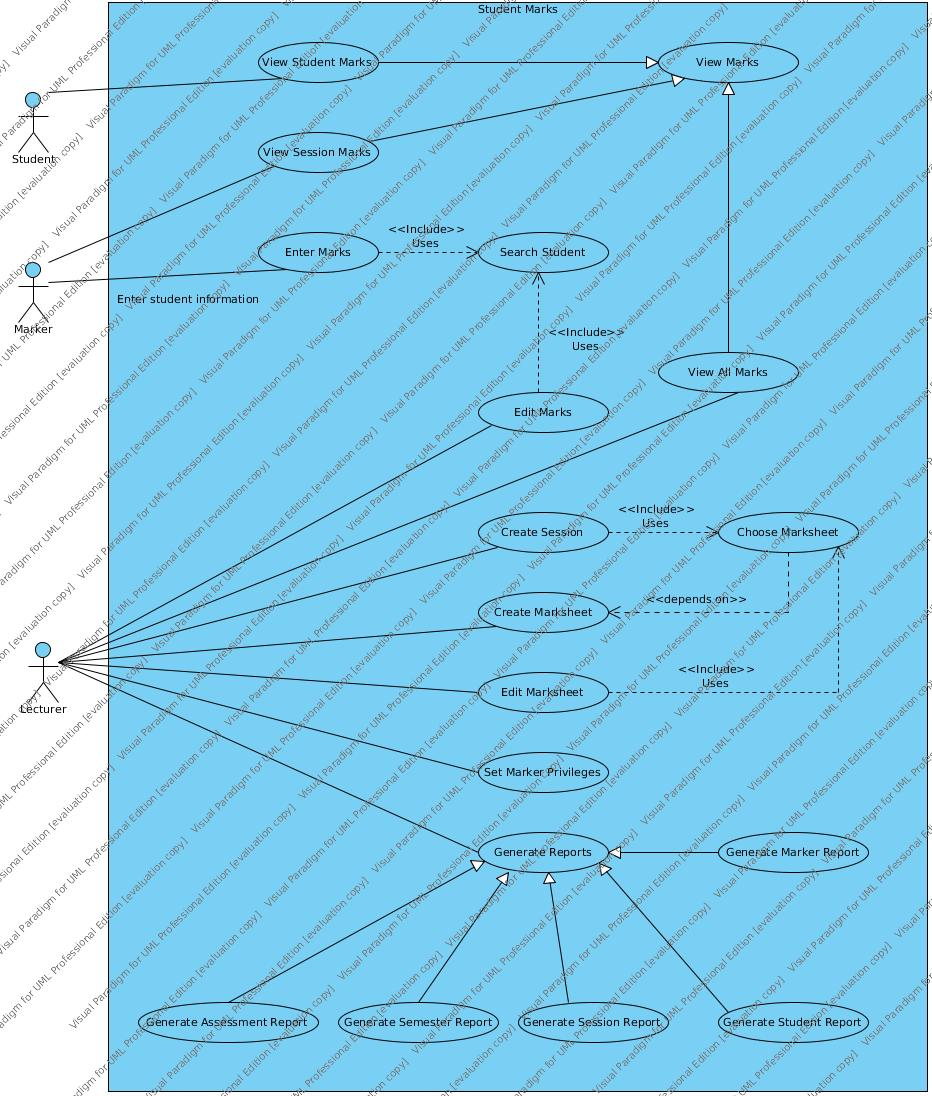
\includegraphics[height=15cm]{StudentMarks}
			\end{figure}

		\subsection{Required Functionality}

		\subsection{Use Case Prioritisation}

		\subsection{Use Case/Service Contracts}

		\subsection{Process Specification}

		\subsection{Domain Objects}

	\section{Open Issues}

	\section{Glossary}
>>>>>>> Inserted UML diagram as a figure

\end{document}